
\chapter{Projekt i implementacja strony serwerowej opartej na architekturze REST w technologi Django oraz bazy danych MySQL}
\section{Narzędzia i techonologie}
\subsection{Django}
Django~\cite{Django} jest darmową, wysokopoziomową platformą programistyczną przeznaczoną do tworzenia aplikacji internetowych. Dostarcza wiele narzędzi ułatwiających szybką oraz prostą implementację. Oparta jest na wzorcu architektonicznym model-template-view~(zob.~rysunek~\ref{rys:django}). 

\begin{figure}[H]
	\centering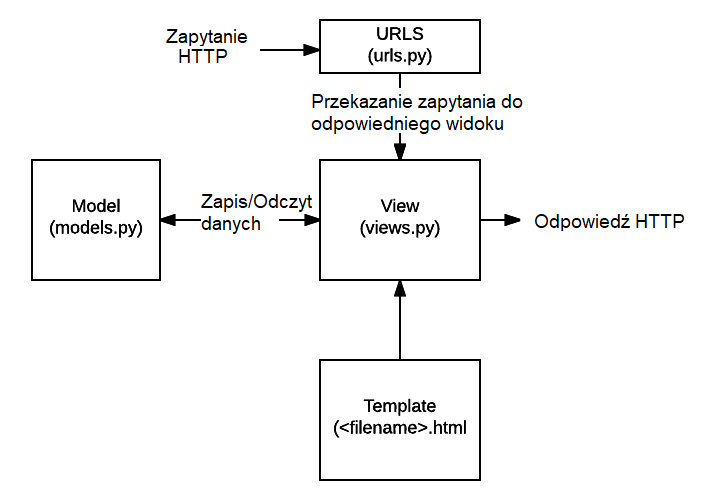
\includegraphics[width=14cm]{figures/DjangoSchemat}
	\caption{Schemat przepływu danych w Django~\cite{DjangoSchemat}}\label{rys:django}
\end{figure}

Napisana jest w języku Python. Jednymi z najważniejszych cech Django są:
\begin{itemize}
	\item łatwy i bezpieczny dostęp do bazy danych,
	\item duża skalowalność oraz wydajność,
	\item wbudowane zabezpieczenia przed popularnymi atakami,
	\item rozbudowana dokumentacja.
\end{itemize}
\subsection{MySQL}
MySQL~\cite{SQL} jest systemem służącym do zarządzania relacyjnymi bazami danych. Model relacyjny zapewnia łatwość w projektowaniu oraz implementacji. Udostępniony jest na licencji wolnego oprogramowania i dostępny jest dla wszystkich popularnych systemów operacyjnych. Bazy danych oparte na tym systemie są wstanie obsługiwać olbrzymie liczby zapytań w bardzo krótkim czasie.
\subsection{MySQL Workbench}
MySQL Workbench~\cite{Workbench} to narzędzie do projektowania, tworzenia oraz zarządzania bazami danych MySQL. Posiada bardzo przejrzysty i intuicyjny interfejs, przez co cieszy się dużą popularnością. Wiele podstawowych czynności takich jak np. tworzenie i edycja tabel, można wykonać bez znajomości zapytań SQL, gdyż są one generowane automatycznie.

\section{Implementacja serwera REST API}
\subsection{REST}
\begin{figure}[H]
	\centering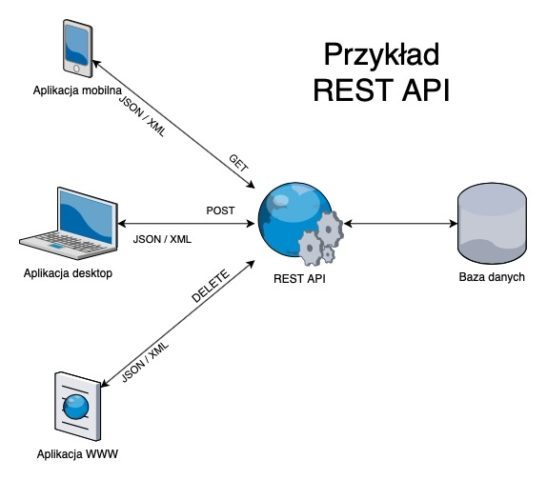
\includegraphics[width=12cm]{figures/rest}
	\caption{Przykładowy schemat działania REST API~\cite{SchematRest}}\label{rys:rest}
\end{figure}
REST ~\cite{REST} jest stylem architektonicznym wprowadzającym pewien standard komunikacyjny dla internetowych systemów informatycznych~(zob.~rysunek~\ref{rys:rest}). Jego najważniejszymi zaletami są szybkość oraz uniwersalność. Interfejsy programistyczne spełniające założenia REST mogą komunikować się z dowolnym urządzeniem sieciowym, pod warunkiem wysyłania przez nie zapytań w odpowiednim formacie. Jednymi z głównych zasad tego stylu są:
\begin{itemize}
	\item zastosowanie modelu klient-serwer,
	\item bezstanowość,
	\item wykorzystywanie pamięci cache przeglądarki w celu zapamiętywania odpowiedzi,
	\item interfejs programistyczny jednolity dla każdej aplikacji klienckiej.
\end{itemize}
Zapytania zazwyczaj wysyłane są przy pomocy protokołu HTTP. Zarówno do zapytań, jak i do odpowiedzi, najczęściej wykorzystywane są metody GET oraz POST. Informacje przesyłane między klientem a serwerem muszą być precyzyjne, zwykle występują one w formacie JSON. 

\subsection{Modele}
Jednym z najważniejszych mechanizmów zaimplementowanych w Django są modele. Są one swego rodzaju mapowaniem klas języka Python na tabele bazy danych. Takie rozwiązanie zapewnia bardzo szybki i wygodny dostęp do przechowywanych informacji. Klasy te zdefiniowane są w pliku ,,models.py''. Wykorzystując wbudowane funkcje wykorzystywanej platformy programistycznej, można zarówno wygenerować tabele bazy danych na podstawie modeli, jak i wygenerować modele na podstawie gotowych tabel.

W projekcie znajduje się następujących siedem modeli: 
\begin{itemize}
	\item Classrooms,
	\item Lessons,
	\item Planners,
	\item Polls,
	\item Subjects,
	\item Teachers,
	\item Timetables.
\end{itemize}
Każdy odpowiada jednej tabeli z bazy danych, pola w każdej z klas są analogiczne do kolumn w odpowiednich tabelach. Zawierają informacje takie jak np. typ danych, maksymalna długość oraz klucz główny.
Implementacja przykładowej klasy przedstawiona na listingu ~\ref{lst:teachers}

\begin{lstlisting}[caption=Implementacja klasy Teachers, label={lst:teachers}]
	class Teachers(models.Model):
	'''This class represents table that hold information about teachers '''
	teacheremail = models.CharField(db_column='teacherEmail', primary_key=True, max_length=255)
	teachername = models.CharField(db_column='teacherName', max_length=255)
	teachsubject = models.CharField(db_column='teachSubject', max_length=255)
	planneremail = models.CharField(db_column='plannerEmail', max_length=255)
	
	class Meta:
	managed = False
	db_table = 'Teachers'
\end{lstlisting}

\subsection{Adresy internetowe}
Kolejnym elementem implementacji są adresy internetowe. W pliku ,,urls.py'' określone zostały wykorzystywane w projekcie adresy URL, oraz funkcje, które mają zostać wywołane w przypadku otrzymania od klienta zapytania na dany adres. Implementacja adresów przedstawiona została na listingu ~\ref{lst:URLs}
\begin{lstlisting}[caption=Implementacja adresów URL, label={lst:URLs}]
	urlpatterns = [
	path('admin/', admin.site.urls),
	path('api/auth/signup/', views.add_user),
	path('api/auth/signin/', views.get_user),
	path('api/add/subject', views.add_subject),
	path('api/add/teacher', views.add_teacher),
	path('api/add/classroom', views.add_classroom),
	path('api/add/class', views.add_class),
	path('api/get/all/subjects', views.get_subjects),
	path('api/get/all/teachers', views.get_teachers),
	path('api/get/all/classrooms', views.get_classrooms),
	path('api/get/all/classes', views.get_classes),
	path('api/sendEmail', views.send_email),
	path('api/polls/<int:pollNumber>', views.add_poll_data),
	path('api/generatePlan', views.generate_plan),
	path('api/delete/subject', views.del_subject),
	path('api/delete/teacher', views.del_teacher),
	path('api/delete/classroom', views.del_classroom),
	path('api/delete/class', views.del_class),
	path('api/edit/subject', views.edit_subject),
	path('api/edit/teacher', views.edit_teacher),
	path('api/edit/classroom', views.edit_classroom),
	path('api/edit/class', views.edit_class),
	path('api/get/plans/class', views.get_classes_timetable),
	path('api/get/plans/classroom', views.get_classrooms_timetable),
	path('api/get/plans/teacher', views.get_teachers_timetable)
	]
\end{lstlisting}
W przypadku, jeśli zapytanie przyjdzie na niezadeklarowany adres, zwrócony zostanie komunikat HTTP z kodem 404(Page Not Found).

\subsection{Widoki}
Widoki to nic innego, jak funkcję języka Python wykonywane w momencie odbioru zapytania przez serwer. Kiedy klient wyśle zapytanie na dany adres, Django sprawdza, czy jest on zadeklarowany we wspomnianym wcześniej pliku ,,urls.py'', jeśli tak, to wywoływana jest odpowiednia funkcja z pliku ,,views.py'' wraz z jej parametrem którym jest samo zapytanie. Dzięki takiej parametryzacji, widok ma łatwy dostęp do otrzymanych informacji, sprawdza on czy są one prawidłowe, oraz wykonuje na nich odpowiednie działania. W tym projekcie, w większości przypadków wykonywane są operacje zapisu i odczytu z bazy danych. Do komunikacji wykorzystywane są metody GET oraz POST z protokołu HTTP.
Implementacje przykładowych widoków obsługujacych zapytania dla danych metod HTTP przedstawione zostały na listingach ~\ref{lst:GetSubjects} oraz ~\ref{lst:AddSubject}
\begin{lstlisting}[caption=Widok obsługujący zapytanie typu GET, label={lst:GetSubjects}]
	@csrf_exempt
	def get_subjects(request):
	''' A function that returns a list of subjects for a given user  '''
	if request.method == 'GET':
	payload = request.headers.get('x-access-token')
	print(payload)
	try:
	user_data = jwt.decode(payload, None, None)
	array = Subjects.objects.filter(planneremail = user_data['email'])
	subjects_list = []
	for i in array:
	subjects_list.append({'subject_name': i.subjectname})
	print(subjects_list)
	response=json.dumps(subjects_list)
	return HttpResponse(response, content_type='text/json')
	except Exception as exc:
	response = json.dumps({'message': str(exc)})
	return HttpResponse(response, content_type='text/json')
\end{lstlisting}

\begin{lstlisting}[caption=Widok obsługujący zapytanie typu POST, label={lst:AddSubject}]
	@csrf_exempt
	def add_subject(request):
	'''Function that takes new subject request and returns response with the appropriate message,
	depending on whether the addition of a subject was successful    '''
	if request.method == 'POST':
	payload = json.loads(request.body)
	name = payload['subject_name']
	token = payload['token']
	try:
	user_data = jwt.decode(token, None, None)
	subject = Subjects(subjectname = name, planneremail = user_data["email"])
	subject.save(force_insert = True)
	response=json.dumps({'message': 'Pomyslnie dodano lekcje'})
	return HttpResponse(response, content_type='text/json')
	except Exception as exc:
	response = json.dumps({'message': str(exc)})
	return HttpResponse(response, content_type='text/json')
\end{lstlisting}

\section{Główne funkcjonalności}
\subsection{Rejestracja i logowanie}
Rejestracja oraz logowanie zrealizowane są za pomocą dwóch adresów, co za tym idzie również dwóch widoków, obsługujących zapytania z metodą POST. Do zarejestrowania nowego użytkownika wymagane jest podanie danych takich informacji jak adres e-mail, login oraz hasło. Funkcja obsługująca rejestrację zapisuje te dane do odpowiedniej tabeli, pod warunkiem że dany użytkownik nie istnieje już w bazie danych, a następnie zwraca odpowiedni komunikat. W przypadku logowania wymagane jest podanie adresu e-mail oraz hasła podanych przy rejestracji. Jeśli podane dane są poprawne, generowany oraz zwracany klientowi jest token (JWT). Zakodowane w nim są wszystkie dane podane przy rejestracji, co pozwala na identyfikację użytkownika przy dalszej komunikacji. Generacja JWT na listingu ~\ref{lst:JWT}. 

\begin{lstlisting}[caption=Widok obsługujący zapytanie typu POST, label={lst:JWT}]
user = Planners.objects.get(planneremail=get_email, password=get_password)


access_token_payload = {
	'email': user.planneremail,
	'login': user.login,
	'password': user.password
}

token = jwt.encode(access_token_payload, settings.SECRET_KEY, algorithm='HS256').decode('utf-8')
\end{lstlisting}

\subsection{Uzupełnianie danych potrzebnych do generacji planu}
Dane które są wymagane do generacji planu lekcji, można podzielić na 4 grupy:
\begin{itemize}
	\item nauczyciele,
	\item klasy,
	\item sale lekcyjne,
	\item przedmioty.
\end{itemize}

W projekcie zaimplementowane są widoki, pozwalające dodawać, edytować, usuwać oraz zwracać informacje o każdej z tych grup. W większości przypadków są to proste operacje zapisu i odczytu z bazy danych, jednak w przypadku dodawania informacji o nauczycielach istnieje dodatkowa funkcjonalność, pozwalająca na wysłanie do nich wiadomości e-mail z adresem do indywidualnej ankiety, w której można określić preferowane godziny pracy. Przy pomyślnej realizacji zapytania o wysłanie wiadomości e-mail, w bazie danych tworzone są wiersze, do których zapisane będą dane z ankiet. Są one identyfikowane po unikatowym numerze, przekazywanym jako parametr w adresie URL. Dzięki takiemu rozwiązaniu, generowany jest indywidualny link do ankiety dla każdego nauczyciela.
\subsection{Generacja oraz zwracanie planów}
Generacja oraz zwracanie planów zrealizowane są za pomocą czterech widoków. Funkcja generacji planu ma za zadanie odczytać wszystkie potrzebne informacje i w odpowiednim formacie przekazać je do generatora. Ze względu na to, że klient nie powinien oczekiwać na odpowiedź oraz że czas generacji planu może być stosunkowo długi, widok ten w przypadku pomyślnego przygotowania danych wejściowych, zwraca informację o rozpoczęciu generacji planu, nie czekając na zakończenie procesu. Dzięki temu, proces generacji nie zaburza połączenia klient-serwer. Kiedy generator skończy pracę, plany lekcji zapisywane są w bazie danych w trzech wersjach, z perspektywy: klas, nauczycieli oraz sal lekcyjnych.
Każdy z tych planów, jest zwracany za pomocą pozostałych trzech widoków.

\section{Baza danych MySQL}
Baza danych składa się z siedmiu tabel. Więszkość wykorzystywanych relacji to ``jeden do wielu''.
Tabela przechowująca dane użytkowników (Planistów) nazywa się ``Planners''. Zawiera ona następujące kolumny:
\begin{itemize}
	\item plannerEmail - adres email planisty (klucz główny),
	\item login - nazwa planisty,
	\item password - hasło planisty.
\end{itemize}

Kolejne tabele zawierają informacje potrzebne algorytmowi do wygenerowania planu. Pierwszą z nich jest tabela ``Subjects''. Zawiera ona listę przedmiotów, dodanych przez danego planistę. Jest to pierwsza z relacji, która zwiera złożony klucz główny, tzn. taki który składa się z więcej niż jednej kolumny. Dane przechowywane są w następujący sposób:
\begin{itemize}
	\item subjectName - nazwa przedmiotu (klucz główny),
	\item plannerEmail - adres email planisty (klucz główny oraz klucz obcy).
\end{itemize}

Podążając za przyjętą w projekcie kolejnością uzupełniania danych, następną tabelą jest ``Teachers'', przechowująca informacje o nauczycielach. Występują w niech następujące kolumny:
\begin{itemize}
 	\item teacherEmail - adres email nauczyciela (klucz główny),
 	\item plannerEmail - adres email planisty (klucz główny oraz klucz obcy),
 	\item teacherName - imie oraz nazwisko nauczyciela,
 	\item teachSubject - przedmioty które prowadzi dany nauczyciel.
\end{itemize}

Rekordy kolejnej tabeli zawierają informację o dostępnych salach lekcyjnych. Nazywa się ona "Classrooms". Podobnie jak dwie poprzednie, ta również zawiera klucz główny złożony z dwóch kolumn. Występują w niej następujące dane:
\begin{itemize}
	\item classroomId - identyfikator sali lekcyjnej (klucz główny),
	\item plannerEmail - adres email planisty (klucz główny oraz klucz obcy),
	\item prefferedSubject - przedmioty, dla których dedykowana jest dana sala.
\end{itemize}

Ostatnią tabelą zawierającą dane wymagane do wygenerowania planu lekcji jest tabela "Lessons". Zawiera ona informacje o klasach. Jako jedyna tabela, posiada klucz główny składający się aż z trzech kolumn. Przechowywane w niej są następujące dane:
\begin{itemize}
	\item className - nazwa klasy (klucz główny),
	\item subjectName - nazwa przedmiotu (klucz główny oraz klucz obcy),
	\item plannerEmail - adres email planisty (klucz główny oraz klucz obcy),
	\item lesssonCount - liczba godzin danego przedmiotu w tygodniu,
	\item teacherEmail - adres email nauczyciela (klucz obcy).
\end{itemize}

Poza powyższymi tabelami, przechowywującymi informacje konieczne do wygenerowania planu, jest jeszcze taka, która zawiera informacje na temat preferowanych godzin pracy danych nauczycieli. Dane te, są opcjonalne. Tabela nosi nazwę "Polls", a jej kolumny wyglądają następująco:
\begin{itemize}
	\item plannerEmail - adres email planisty (klucz główny oraz klucz obcy),
	\item teacherEmail - adres email nauczyciela (klucz główny oraz klucz obcy),
	\item teacherPref -  dane dotyczące preferowanych godzin pracy nauczyciela,
	\item pollId - numer ankiety, wykorzystywany do generacji odpowiedniego adresu URL.
\end{itemize}
 
Ostania tabela w bazie danych nazywa się "Timetables". Przechowuje ona wygenerowane plany lekcji. Jej struktura wygląda następująco:
\begin{itemize}
	\item plannerEmail - adres email planisty (klucz główny oraz klucz obcy),
	\item ClassesTimetable - plan lekcji z punktu widzenia klas,
	\item TeachersTimetable -  plan lekcji z punktu widzenia nauczyciela,
	\item ClassroomsTimetable -plan lekcji z punktu widzenia sal lekcyjnych.
\end{itemize}

Diagram związków encji opisanej bazy danych, znajduje się na rysunku ~\ref{rys:sqldiag}

\begin{figure}[H]
	\centering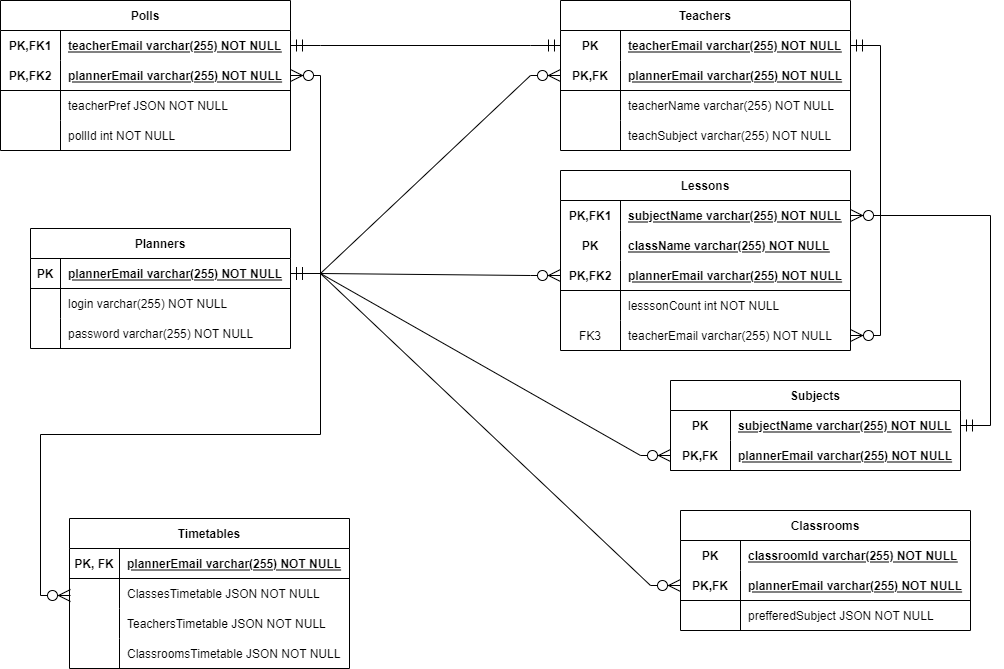
\includegraphics[width=\textwidth]{figures/SQLdiag}
	\caption{Diagram związków encji}\label{rys:sqldiag}
\end{figure}